\chapter[SNAFU generates ULP CGRAs]{SNAFU generates ULP CGRAs\raisebox{.3\baselineskip}{\normalsize\cref{snafu:cite1}}}
\footnotetext[1]{\label{snafu:cite1}\cite{snafu} G. Gobieski, A. O. Atli, K. Mai, B. Lucia, and N. Beckmann, ``SNAFU: an ultra-low-power, energy-minimal CGRA-generation framework and architecture,'' in 2021 ACM/IEEE 48th Annual International Symposium on Computer Architecture (ISCA). IEEE, 2021, pp. 1027–1040.}
\label{chapter:snafu}

\newcommand{\snafuframe}{\snafu}
\newcommand{\snafuarch}{{\protect\fauxsc{Snafu-Arch}}\xspace}
\newcommand*\circled[1]{\tikz[baseline=(char.base)]{\node[shape=circle,draw,inner sep=0.5pt] (char) {#1};}}
\newcommand{\bigemph}[1]{\emph{\bfseries #1}}
\newcommand{\ucore}{\textmu core\xspace}
\newcommand{\ucfg}{\textmu cfg\xspace}

\newcommand{\figSNAFUMotivate}{
\begin{figure}[t]
	\centering
	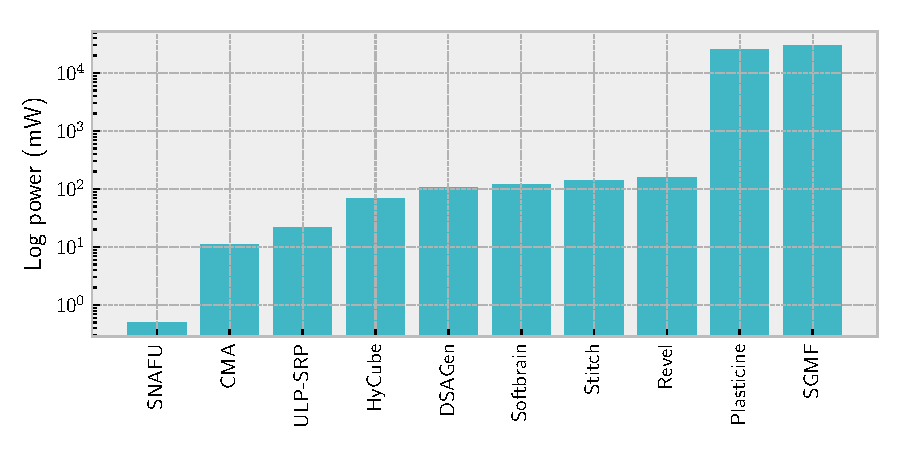
\includegraphics[width=\columnwidth]{snafu/figures/pdf/motivate.pdf}
	\caption{\snafuframe generates ultra-low-power CGRA fabrics that operate in a power regime not well explored by existing CGRAs.}
	\label{fig:motivate}
\end{figure}
}

\newcommand{\figSNAFUOverviewFramework}{
\begin{figure}[t]
	\centering
	\includegraphics[width=.65\columnwidth]{snafu/figures/pdf/overview.pdf}
	\caption{Overview of \snafu. \snafuframe is a flexible framework for generating ULP CGRAs. It takes a {\em bring-your-own functional unit} approach, allowing the designer to easily integrate custom logic tailored for specific domains.}
	\label{fig:overview:framework}
\end{figure}
}

\newcommand{\figSNAFUOverviewExecute}{
\begin{figure*}[t]
	\centering
	\includegraphics[width=\linewidth]{snafu/figures/pdf/execute.pdf}
	\caption{An example execution on a \snafuframe CGRA fabric. The DFG is extracted from vectorized C-code, compiled to a bitstream, and then executed according to asynchronous dataflow firing.}
	\label{fig:overview:execute}
\end{figure*}
}

\newcommand{\figSNAFUCompilation}{
\begin{figure}[htb]
	\centering
	\includegraphics[width=.9\columnwidth]{snafu/figures/pdf/compilation.pdf}
	\caption{Compiler extracts dataflow graphs from vectorized C-code and uses an integer linear program to optimally map the dataflow graph to specific PEs and routes in the CGRA fabric.}
	\label{fig:compilation}
\end{figure}
}

\newcommand{\figSNAFUArch}{
\begin{figure}[t]
	\centering
	\includegraphics[width=.65\columnwidth]{snafu/figures/pdf/arch.pdf}
	\caption{Architectural diagram of \snafuarch. \snafuarch possesses a RISC-V scalar core tightly coupled with the \snafuframe fabric. Both are attached to a unified 256\,KB banked memory.}
	\label{fig:arch}
\end{figure}
}

\newcommand{\figSNAFUPE}{
\begin{figure}[t]
	\centering
	\includegraphics[width=.65\columnwidth]{snafu/figures/pdf/pe.pdf}
	\caption{\snafuframe provides a standardized interface that makes integrating new types of PEs trivial. \snafuframe handles variable-latency logic, PE-specific configuration, and the sending and receiving of values from the on-chip network.}
	\label{fig:pe}
\end{figure}
}

\newcommand{\figSNAFUDie}{
\begin{figure}[t]
	\centering
	\includegraphics[width=.9\columnwidth]{snafu/figures/pdf/die.pdf}
	\caption{Layout of \snafuarch. Memory PEs are blue, scratchpad PEs are green, basic-ALU PEs are red, multiplier PEs are purple, the scalar core is yellow, and main-memory control logic is orange. The remaining grey regions contain routers and wires. }
	\label{fig:die}
\end{figure}
}

\newcommand{\figSNAFUPerf}{
\begin{figure}[htb]
	\centering
	\includegraphics[width=.9\columnwidth]{snafu/figures/pdf/perf-graph-crop.pdf}
	\caption{\snafu}
	\label{fig:perf:alone}
\end{figure}
}

\newcommand{\figSNAFUTopResults}{
	\begin{figure}[t]
		\centering
		\includegraphics[width=0.7\linewidth]{snafu/figures/pdf/energy_all_norm_legend-graph-crop.pdf}\\
		\vspace{0.4em}
		\begin{subfigure}{0.49\linewidth}
			\centering
			\includegraphics[width=0.8\linewidth]{snafu/figures/pdf/energy_avg-graph-crop.pdf}
			\caption{Energy savings.}
			\label{fig:top:energy}
		\end{subfigure}
		\begin{subfigure}{0.49\linewidth}
			\centering
			\includegraphics[width=0.8\linewidth]{snafu/figures/pdf/perf_overall-graph-crop.pdf}
			\caption{Avg performance.}
			\label{fig:top:perf}
		\end{subfigure}
		\caption{Average normalized energy and speedup (normalized to the scalar baseline). \snafuarch uses $81\%$ less energy and is $9.9\times$ faster than the scalar baseline.}
		\label{fig:top}	
	\end{figure}
}

\newcommand{\figSNAFUPrimaryResults}{
	\begin{figure*}[t]
		\centering
		\includegraphics[width=0.5\linewidth]{snafu/figures/pdf/energy_all_norm_legend-graph-crop.pdf}\\
		\vspace{0.4em}

		\begin{subfigure}{0.49\linewidth}
			\centering
			\includegraphics[width=\linewidth]{snafu/figures/pdf/energy_all_norm-graph-crop.pdf}
			\caption{Energy}
			\label{fig:energy:norm}
		\end{subfigure}
		\hfill
		\begin{subfigure}{0.5\linewidth}
			\centering
			\includegraphics[width=\linewidth]{snafu/figures/pdf/perf_all-graph-crop.pdf}
			\caption{Execution time}
			\label{fig:perf}
		\end{subfigure}
		\caption{Energy and execution time, normalized to the scalar baseline, across ten applications on large inputs. On average, \snafuarch uses $81\%$, $57\%$, $41\%$ less energy and is $9.9\times$, $3.2\times$, and $4.4\times$ faster than the scalar design, vector baseline, and \manic, respectively.
                }

		\label{fig:primary}
	\end{figure*}
}

\newcommand{\figSNAFUCacheNorm}{
\begin{figure}[htb]
	\centering
	\includegraphics[width=0.7\columnwidth]{snafu/figures/pdf/energy_all_norm_legend-graph-crop.pdf}\\
	\vspace{0.4em}
	\includegraphics[width=.9\columnwidth]{snafu/figures/pdf/cache_norm-graph-crop.pdf}
	\caption{\snafu}
	\label{fig:cache:norm:alone}
\end{figure}
}

\newcommand{\figSNAFUBufNorm}{
\begin{figure}[htb]
	\centering
	\includegraphics[width=0.7\columnwidth]{snafu/figures/pdf/energy_all_norm_legend-graph-crop.pdf}\\
	\vspace{0.4em}
	\includegraphics[width=.9\columnwidth]{snafu/figures/pdf/buf_norm-graph-crop.pdf}
	\caption{\snafu}
	\label{fig:buf:norm:alone}
\end{figure}
}

\newcommand{\figSNAFUInputEnergy}{
\begin{figure}[htb]
	\centering
	\includegraphics[width=.9\columnwidth]{snafu/figures/pdf/size_norm-graph-crop.pdf}
	\caption{\snafuarch}
	\label{fig:size:energy:alone}
\end{figure}
}

\newcommand{\figSNAFUInputPerf}{
\begin{figure}[htb]
	\centering
	\includegraphics[width=.9\columnwidth]{snafu/figures/pdf/size_perf-graph-crop.pdf}
	\caption{\snafuarch}
	\label{fig:size:perf:alone}
\end{figure}
}

\newcommand{\figSNAFUSensUnrollResults}{
\begin{figure*}[t]
	\centering
	\includegraphics[width=0.5\linewidth]{snafu/figures/pdf/energy_all_norm_legend-graph-crop.pdf}\\
	\vspace{0.4em}
	\begin{minipage}{0.31\linewidth}
		\begin{subfigure}[t]{0.49\linewidth}
			\centering
			\includegraphics[height=1in]{snafu/figures/pdf/sens_size_energy-graph-crop.pdf}
			\caption{Energy.}
			\label{fig:sens:size:energy}
		\end{subfigure}
		\hfill
		\begin{subfigure}[t]{0.49\linewidth}
			\centering
			\includegraphics[height=1in]{snafu/figures/pdf/sens_size_perf-graph-crop.pdf}
			\caption{Speedup.}
			\label{fig:sens:size:perf}
		\end{subfigure}
		\vspace{1.1em}
		\caption{\snafuarch vs.\ the scalar design across three input sizes -- small (S), medium (M) and large (L).}
		\label{fig:sens:size}
	\end{minipage}
        \hfill
	\begin{minipage}{0.67\linewidth}
		\begin{subfigure}[t]{0.49\columnwidth}
			\centering
			\includegraphics[width=0.99\linewidth]{snafu/figures/pdf/case_unroll_norm-graph-crop.pdf}
			\caption{Energy.}
			\label{fig:unroll:energy}
		\end{subfigure}
		\hfill
		\begin{subfigure}[t]{0.49\columnwidth}
			\centering
			\includegraphics[width=0.99\linewidth]{snafu/figures/pdf/case_unroll_perf-graph-crop.pdf}
			\caption{Speedup.}
			\label{fig:unroll:perf}
		\end{subfigure}
		\caption{Energy and speedup of \manic, un\manic (w/ loop unrolling), \snafuarch, and un\snafuarch (w/ loop unrolling), normalized to \snafuarch. un\snafuarch uses $31\%$ less energy and is $2.2\times$ faster \snafuarch; \manic benefits much less.}
		\label{fig:unroll}
	\end{minipage}
	\label{fig:sens}
\end{figure*}
}

\newcommand{\figSNAFUUnrollEnergy}{
\begin{figure}[htb]
	\centering
	\includegraphics[width=.9\columnwidth]{snafu/figures/pdf/case_unroll_norm-graph-crop.pdf}
	\caption{Energy}
\end{figure}
}

\newcommand{\figSNAFUUnrollPerf}{
\begin{figure}[htb]
	\centering
	\includegraphics[width=.9\columnwidth]{snafu/figures/pdf/case_unroll_perf-graph-crop.pdf}
	\caption{\snafuarch}
	\label{fig:unroll:perf:alone}
\end{figure}
}

\newcommand{\figSNAFUUnrollResults}{
	\begin{figure}[t]
		\centering
		\includegraphics[width=0.9\columnwidth]{snafu/figures/pdf/energy_all_norm_legend-graph-crop.pdf}\\
		\vspace{0.4em}
		\begin{subfigure}{0.49\columnwidth}
			\centering
			\includegraphics[width=\linewidth]{snafu/figures/pdf/case_unroll_norm-graph-crop.pdf}
			\caption{Energy.}
			\label{fig:unroll:energy}
		\end{subfigure}
		\hfill
		\begin{subfigure}{0.49\columnwidth}
			\centering
			\includegraphics[width=\linewidth]{snafu/figures/pdf/case_unroll_perf-graph-crop.pdf}
			\caption{Speedup.}
			\label{fig:unroll:perf}
		\end{subfigure}
		\caption{Energy and speedup of \manic, un\manic (w/ loop unrolling), \snafuarch, and un\snafuarch (w/ loop unrolling), normalized to \snafuarch. un\snafuarch uses $31\%$ less energy and is $2.2\times$ faster \snafuarch; \manic benefits much less.}
		\label{fig:unroll}
	\end{figure}
}

\newcommand{\figSNAFUAccel}{
	\begin{figure*}[t]
		\centering
		\includegraphics[width=.5\linewidth]{snafu/figures/pdf/case_dmm_energy_legend-graph-crop.pdf}\\
		\vspace{0.4em}

		\begin{subfigure}{0.32\linewidth}
			\centering
			\includegraphics[width=\linewidth]{snafu/figures/pdf/case_dmm_annotated-crop.pdf}
			\caption{DMM energy.}
			\label{fig:accel:dmm}
		\end{subfigure}
		\begin{subfigure}{0.32\linewidth}
			\centering
			\includegraphics[width=\linewidth]{snafu/figures/pdf/case_sort_annotated-crop.pdf}
			\caption{Sort energy.}
			\label{fig:accel:sort}
		\end{subfigure}
		\begin{subfigure}{0.32\linewidth}
			\centering
			\includegraphics[width=\linewidth]{snafu/figures/pdf/case_fft_annotated-crop.pdf}
			\caption{FFT energy.}
			\label{fig:accel:fft}
		\end{subfigure}

		\caption{Quantifying the cost of \snafu's programmability on three benchmarks. Each subfigure shows, from left-to-right, the effect of gradually removing \snafuarch's programmability and increasing its specialization, culminating in a hand-coded ASIC. Overall, \snafuarch's energy is within $2.6\times$ on average of the ASICs', and can be easily specialized to narrow the gap at low upfront design cost.}
		\label{fig:accel}
	\end{figure*}
}

\newcommand{\figSNAFUScratchEnergy}{
\begin{figure}[t]
	\centering
	\includegraphics[width=.9\columnwidth]{snafu/figures/pdf/case_scratch_norm-graph-crop.pdf}
	\caption{\snafuarch}
	\label{fig:scratch:energy:alone}
\end{figure}
}

\newcommand{\figSNAFUScratchPerf}{
\begin{figure}[htb]
	\centering
	\includegraphics[width=.9\columnwidth]{snafu/figures/pdf/case_scratch_perf-graph-crop.pdf}
	\caption{\snafuarch}
	\label{fig:scratch:perf:alone}
\end{figure}
}

\newcommand{\figSNAFUScratchResults}{
	\begin{figure}[t]
		\centering
		\includegraphics[width=0.9\columnwidth]{snafu/figures/pdf/energy_all_norm_legend-graph-crop.pdf}\\
		\vspace{0.4em}
		\begin{subfigure}{0.49\columnwidth}
			\centering
			\includegraphics[width=\linewidth]{snafu/figures/pdf/case_scratch_norm-graph-crop.pdf}
			\caption{Energy.}
			\label{fig:scratch:energy}
		\end{subfigure}
		\hfill
		\begin{subfigure}{0.49\columnwidth}
			\centering
			\includegraphics[width=\linewidth]{snafu/figures/pdf/case_scratch_perf-graph-crop.pdf}
			\caption{Speedup.}
			\label{fig:scratch:perf}
		\end{subfigure}
		\caption{Energy and speedup of \manic, \snafuarch w/ and w/out scratchpads, normalized to \snafuarch. Scratchpads improve energy-efficiency by $34\%$ and performance by $13\%$.}
		\label{fig:scratch}
	\end{figure}
}

\newcommand{\tabSNAFUParams}{
  \begin{table}
    %% \renewcommand{\tabSNAFUcolsep}{12pt}
%% \footnotesize
\centering
%% \resizebox{\linewidth}{!}{
\begin{tabular}{ccp{1.5in}r}
\toprule
 &  & \textbf{Parameter}       & \textbf{Values} \\
\midrule
 &  & Frequency		       & 50 MHz          \\
 &  & Main memory              & 256\,KB         \\
 &  & Scalar register \#       & 16		 \\[.5ex]
\midrule
\multirow{3}{.5em}{\rotatebox{90}{Vector}}
 &  & Vector register \#       & 16              \\
 &  & Vector length            & 16/32/64        \\
 &  & Window size (for \manic) & 8               \\[.5ex]
\midrule
\multirow{5}{.5em}{\rotatebox{90}{\snafuarch}}
 &  & Fabric dimensions	       & 6$\times$6	 \\
 &  & Memory PE \#    	       & 12		 \\
 &  & Basic-ALU PE \#          & 12		 \\
 &  & Multiplier PE \#         & 4		 \\
 &  & Scratchpad PE \#         & 8		 \\[.5ex]
\bottomrule
\end{tabular}
%}
\caption{Microarchitectural parameters.}
\label{tab:params}
\end{table}
}

\newcommand{\tabSNAFUApp}{
  \begin{table}[t]
\footnotesize
\centering
\resizebox{\linewidth}{!}{
\begin{tabular}{lp{1.25in}p{0.3in}p{0.3in}p{0.325in}}
\toprule
\textbf{Name} & \textbf{Description}                                      & \textbf{Small}                    & \textbf{Medium}                   & \textbf{Large}                    \\
\midrule
\bf FFT       & 2D Fast-fourier transform                                 & 16$\times$16                      & 32$\times$32                      & 64$\times$64                      \\
\bf DWT       & 2D Discrete wavelet trnsfrm                               & 16$\times$16                      & 32$\times$32                      & 64$\times$64                      \\
\bf Viterbi   & Viterbi decoder                                           & 256                               & 1024                              & 4096                              \\
\bf Sort      & Radix sort                                                & 256                               & 512                               & 1024                              \\
\bf SMM       & Sparse matrix-matrix                                      & 16$\times$16                      & 32$\times$32                      & 64$\times$64                      \\
\bf DMM       & Dense matrix-matrix                                       & 16$\times$16                      & 32$\times$32                      & 64$\times$64                      \\
\bf SMV       & Sparse matrix-dense vector                                & 32$\times$32                      & 64$\times$64                      & 128$\times$128                    \\
\bf DMV       & Dense matrix-dense vector                                 & 32$\times$32                      & 64$\times$64                      & 128$\times$128                    \\
\bf Sconv     & Sparse 2D convolution \newline \mbox{}\quad {\em filter:} & 16$\times$16, \newline 3$\times$3 & 32$\times$32, \newline 5$\times$5 & 64$\times$64, \newline 5$\times$5 \\
\bf Dconv     & Dense 2D convolution \newline \mbox{}\quad {\em filter:}  & 16$\times$16, \newline 3$\times$3 & 32$\times$32, \newline 5$\times$5 & 64$\times$64, \newline 5$\times$5 \\
\bottomrule
\end{tabular}
}
\caption{Benchmarks and their input sizes.}
\label{tab:app}
  \end{table}
}

\newcommand{\tabSNAFUTabs}{
	\tabSNAFUParams
	\tabSNAFUApp
}

\newcommand{\figSNAFUIntroOverview}{
	\begin{figure}
		\centering
		\includegraphics[width=0.75\linewidth]{snafu/figures/pdf/intro.pdf}
		\caption{\snafuframe is an ULP CGRA-generation framework and architecture. It converts a flexible abstract specification of a CGRA to synthesizable RTL. \snafuarch is an instantiation that integrates a $6\times6$ \snafuframe fabric with an ULP core and on-chip memory.}
		\label{fig:intro:overview}
	\end{figure}
}  

\newcommand{\figSNAFUIntroLayout}{
	\begin{figure}
		\centering
	        \includegraphics[width=.7\columnwidth]{snafu/figures/pdf/die.pdf}
	        \caption{Layout of \snafuarch, a complete ULP system with CGRA.}
	        \label{fig:intro:layout}
	\end{figure}
}  

\newcommand{\figSNAFUIntro}{
\begin{figure}[t]
	\centering
	\begin{subfigure}{0.49\linewidth}
		\centering
		\includegraphics[width=0.9\linewidth]{snafu/figures/pdf/energy_overall-graph-crop.pdf}
		\caption{Energy savings.}
		\label{fig:intro:energy}
	\end{subfigure}
	\begin{subfigure}{0.49\linewidth}
		\centering
		\includegraphics[width=0.9\linewidth]{snafu/figures/pdf/perf_overall-graph-crop.pdf}
		\caption{Performance.}
		\label{fig:intro:perf}
	\end{subfigure}

	\caption{\snafuarch's energy and performance normalized to a scalar baseline. On average, \snafuframe uses $81\%$ less energy and is $9.9\times$ faster, or $41\%$ less energy and $4.4\times$ faster than \manic.}
	\label{fig:intro}
\end{figure}	
}

\newcommand{\tabSNAFUMotivate}{
  \begin{table*}
  \centering
  \scriptsize
  \resizebox{\linewidth}{!}{
  \begin{tabular}{l|p{0.7in}p{0.7in}p{0.7in}|p{0.7in}p{0.7in}p{0.7in}|p{0.7in}}
    \toprule
                            & \multicolumn{3}{c|}{\bf Ultra-low-power CGRAs} & \multicolumn{3}{c|}{\bf High-performance CGRAs}                                                                                                                                                     \\[.5ex]
                            & \bf ULP-SRP~\cite{srp}                         & \bf CMA~\cite{cma} & \bf IPA~\cite{ipa} & \bf HyCube~\cite{karunaratne2017hycube} & \bf Revel~\cite{weng2020hybrid}    & \bf SGMF~\cite{voitsechov2014single} & \bf \snafu                            \\
    \midrule
    \bf Fabric size         & 3$\times$3                                     & 8$\times$10        & 4$\times$4         & 4$\times$4                              & 5$\times$5                         & 8$\times$8 + 32 mem                  & N$\times$N (6$\times$6 in \snafuarch) \\[.5ex]
    \bf NoC                 & Neighbors only                                 & Neighbors only     & Neighbors only     & Static, bufferless, multi-hop           & Static \& dynamic NoCs (2$\times$) & Dynamic routing                      & Static, bufferless, multi-hop       \\[.5ex]
    \bf PE assignment       & Static                                         & Static             & Static             & Static                                  & Static \emph{or} dynamic           & Dynamic                              & Static                              \\[.5ex]
    \bf Time-share PEs?     & Yes                                            & Yes                & Yes                & Yes                                     & Yes                                & Yes                                  & No                                  \\[.5ex]
    \bf PE firing           & Static                                         & Static             & Static             & Static                                  & Static \emph{or} dynamic           & Dynamic                              & Dynamic                             \\[.5ex]
    \bf Heterogeneous PEs?  & No                                             & No                 & No                 & No                                      & Yes                                & Yes                                  & Yes                                 \\[.5ex]
    \bf Buffering (approx.) & ---                                            & ---                & 188\,B / PE        & 272\,B / PE                             & $\approx$1\,KB / PE                & $\gg$1\,KB / PE                      & 40\,B / PE                          \\[.5ex]
    \midrule
    \bf Power               & 22\,mW                                         & 11\,mW             & 3--5\,mW           & 15--70\,mW                              & 160\,mW                            & 20\,W                                & $<$1\,mW                            \\[.5ex]
    \bf MOPS/mW (approx.)   & 30--100                                        & 100--200           & 140                & 60--90                                  & 60                                 & 60                                   & 305                                 \\[.5ex]
    \bottomrule
  \end{tabular}}
  \caption{Architectural comparison of \snafu to several prior CGRAs.}
  \label{tab:motivation}
\end{table*}
}


The opportunity for tiny, ULP devices is enormous~\cite{lucia2017intermittent}, but enabling sophisticated processing on these devices remains challenging.
% 
Prior chapters have presented progress on this challenge, contributing to a new ULP sensor system stack.
% 
\autoref{chapter:sonic} described software to enable machine inference on commodity MCUs and \autoref{chapter:manic} proposed \manic and \msilicon, a new computer architecture and silicon prototype, respectively.
% 
\manic is an energy-efficient vector-dataflow co-processor that is a big improvement over COTS devices.
% 
However, it stills fall short due to high switching activity
in the shared execution pipeline, a significant inefficiency at ULP-scale.
% 
Eliminating these overheads can reduce energy by nearly half, proving that, despite their low operating power, \manic and other existing programmable ULP designs~\cite{dally:ieee08:elm,hempstead2005ultra,warneke200417,nazhandali2005energy} are not energy-minimal.
% 
Alternatively, custom ASICs would achieve energy-minimality, but come at high upfront cost~\cite{hotmobile2021} and with severely limited application scope, risking quick obsolece.
% 
Thus, there is still a need for new architectures that achieve ULP ($<$1\,mW), \emph{energy-minimal} operation while maintaining a high degree of design flexibility and ease of programmability.

\paragraph{\Ulp CGRAs are the answer}
%
This chapter presents \snafuframe,%
\footnote[2]{\underline{S}imple \underline{N}etwork of \underline{A}rbitrary \underline{F}unctional \underline{U}nits.}
a framework to generate ULP, energy-minimal coarse-grain reconfigurable arrays (CGRAs).
%
\snafuframe CGRAs execute in a \emph{spatial vector-dataflow} fashion,
mapping a dataflow graph (DFG) spatially across a fabric of processing elements (PEs),
applying the same DFG to many input data values,
and routing intermediate values directly from producers to consumers.
%
The insight is that spatial vector-dataflow minimizes instruction and data-movement energy, just like \manic,
but also eliminates unnecessary switching activity because operations do not share execution hardware.

The major difference from most prior CGRAs~\cite{plasticine,dyser,nowatzki:isca17:stream-dataflow,goldstein2000piperench,trips,weng2020dsagen,weng2020hybrid,voitsechov2014single,mishra2006tartan,tan2018stitch,karunaratne2017hycube,voitsechov2018inter,evx} is the extreme design point
--- \snafuframe operates at \emph{orders-of-magnitude lower energy and power budget},
demanding an exclusive focus on energy-minimal design.
%
\snafuframe is designed from the ground up to minimize energy, even at
the cost of area or performance.
%
For example, \snafuframe schedules only one operation per PE, which
minimizes switching activity (energy) but increases the number of PEs needed (area).
%
As a result of such design choices, \snafuframe comes within 2.6$\times$
of ASIC energy efficiency while remaining fully programmable.
%

\snafuframe generates ULP CGRAs from a high-level description of available PEs and the fabric topology.
%
\snafuframe defines a standard PE interface that lets designers \emph{``bring your own function unit''}
and easily integrate it into a ULP CGRA,
along with a library of common PEs.
%
The \snafuframe framework schedules operation execution and routes intermediate values to dependent operations
while consuming minimal energy.
%
\snafuframe is easy to use:
it includes a compiler that maps vectorized C-code to efficient CGRA bitstreams,
and it reduces design effort of tape-out via top-down synthesis of CGRAs.

\figSNAFUIntro

\paragraph{Contributions} This chapter contributes the following:
\begin{compactitem}
\item We present \snafuframe, the first flexible CGRA-generator for ULP, energy-minimal systems.
  \snafuframe makes it easy to integrate new functional units,
  compile programs to energy-efficient bitstreams,
  and produce tape-out-ready hardware.
  
\item We discuss the key design choices in \snafuframe that minimize energy:
  scheduling at most one operation per PE;
  asynchronous dataflow without tag-token matching;
  statically routed, bufferless, multi-hop NoC;
  and producer-side buffering of intermediate values.
  
\item We describe \snafuarch, a complete ULP system-on-chip with a CGRA fabric,
  RISC-V scalar core, and memory.
  We implement \snafuarch in an industrial sub-28\,nm FinFET process with compiled memories.
  \snafuarch operates at $<$1\,mW at 50\,MHz.
  \snafuarch reduces energy by $81\%$ v.\ a scalar core
  and $41\%$ v.\ \manic;
  and improves performance by $9.9\times$ v.\ a scalar core
  and $4.4\times$ v. \manic.

\item Finally, we quantify the cost of programmability through three
  comprehensive case studies that compare \snafuarch against
  fixed-function ASIC designs. We find that programmability comes at
  relatively low cost: on average, \snafuarch takes $2.6\times$ more
  energy and $2.1\times$ more time than an ASIC for the same
  workload. We break down \snafuarch's energy in detail, showing that it
  is possible to close the gap further while retaining significant
  general-purpose programmability. These results call into
  question the need for extreme specialization in most ULP
  deployments.
  
\end{compactitem}
\figSNAFUOverviewFramework
\figSNAFUOverviewExecute
\section{Overview}
\label{snafu:overview}

\snafuframe is a framework for generating energy-minimal, ULP CGRAs
and compiling applications to run efficiently on them.
%
\snafuarch is a complete ULP system featuring a CGRA generated by \snafuframe,
a scalar core, and memory.

\paragraph{\snafuframe is a flexible ULP CGRA generator}
\snafuframe is a general and flexible framework for converting a high-level
description of a CGRA to valid RTL and ultimately to ULP hardware.
% 
\autoref{fig:overview:framework} shows \snafuframe's workflow.
% 
\snafuframe takes two inputs: a library of processing elements (PEs) and a high-level description of the CGRA topology.
% 
\snafuframe lets designers customize the ULP CGRA
%
via a {\em ``bring your own functional unit''} approach,
defining a generic PE interface that makes it easy to add custom logic to a generated CGRA.

With these inputs, \snafuframe generates complete RTL for the CGRA.
% 
This RTL includes a statically routed, bufferless, multi-hop on-chip network parameterized by the topology description.
% 
It also includes hardware to handle variable-latency timing and asynchronous dataflow firing.
%
Finally, \snafuframe simplifies hardware generation by supporting top-down synthesis,
making it easy to go from a high-level CGRA description to a placed-and-routed ULP design ready for tape out.

\paragraph{\snafuarch is a complete ULP, CGRA-based system}
\snafuarch is a specific, complete system implementation that includes a CGRA generated by \snafuframe.
% % 
The CGRA is a 6$\times$6 mesh topology composed of PEs from \snafuframe's standard PE library.
%
\snafuarch integrates the CGRA fabric with a scalar core and 256\,KB of on-chip SRAM main memory.
%
The resulting system executes vectorized, RISC-V programs~\cite{riscv_2019}
with the generality of software and extremely low power consumption ($\approx$300\,\textmu W).  
% 
Compared to the \mbox{RISC-V} scalar core, \snafuarch uses $81\%$ less energy for equal work and is $9.9\times$ faster.
% 
Compared to \manic (a state-of-the-art general-purpose ULP design), \snafuarch uses $41\%$ less energy and is $4.4\times$ faster.
%
Compared to hand-coded ASICs, \snafuarch uses $2.6\times$ more energy and is $2.1\times$ slower.

\paragraph{Example of \snafu in action}
\autoref{fig:overview:execute} shows the workflow to take a simple vectorized kernel and execute it on an ULP CGRA generated by \snafuframe.
%
This kernel multiplies values at address {\tt \&a} by 5 for the elements where the mask {\tt m} is set,
  sums the result, and stores it to address {\tt \&c}.
% 
\snafuframe's compiler extracts the dataflow from the kernel source code and generates a bitstream to configure the CGRA fabric.
%
The scalar core configures the CGRA fabric and kicks off fabric execution using three new instructions ({\tt vcfg}, {\tt vtfr}, {\tt vfence}),
after which the CGRA runs autonomously in SIMD fashion over arbitrarily many input data values.
% 
The fabric executes the kernel using asynchronous dataflow firing:
\begin{compactitem}
\item[\circled{1}]
In the first timestep, the two memory PEs (that load {\tt a[0]} and {\tt m[0]}) are enabled and issue loads.
%
The rest of the fabric is idle because it has no valid input values.
\item[\circled{2}]
The load for {\tt a[0]} completes, but {\tt m[0]} cannot due to a bank conflict.
%
This causes a stall, which is handled transparently by \snafuframe's scheduling logic and bufferless NoC.
%
Meanwhile, the load of {\tt a[1]} begins.
%
\item[\circled{3}]
% 
As soon as the load for {\tt m[0]} completes, the multiply operation can fire because both of its inputs have arrived.
% 
But {\tt m[0] == 0}, meaning the multiply is disabled, so {\tt a[0]} passes through transparently.
%
The load of {\tt a[1]} completes, and loads for {\tt a[2]} and {\tt m[1]} begin.
%
\item[\circled{4}]
%
When the predicated multiply completes, its result is consumed by the fourth PE, which keeps a partial sum of the products.
%
The preceding PEs continue executing in pipelined fashion,
multiplying {\tt a[1]} $\times$ {\tt 5} (since {\tt m[1] == 1}) and loading {\tt a[3]} and {\tt m[2]}.
%
\item[\circled{5}]
%
Finally, a value arrives at the fifth PE, and is stored back to memory in {\tt c[0]}.
%
Execution continues in this fashion until all elements of {\tt a} and {\tt m} have been processed and a final result has been stored back to memory...
\end{compactitem}

\noindent
The next three sections describe \snafuframe.
% 
\autoref{snafuflexible} describes the \snafuframe ULP CGRA-generator.
% 
\autoref{snafuenergy} describes how \snafuframe minimizes energy.
% 
And \autoref{snafuarch} describes \snafuarch.


\section{Designing \snafuframe to maximize flexibility}
\label{snafu:flexible}

\snafuframe is designed to generate CGRAs that minimize energy, maximize
extensibility, and simplify programming. 
%
For the architect, \snafuframe automates synthesis from the top down and
provides a \emph{``bring your own functional unit''} interface, allowing easy
integration of custom FUs into a CGRA.
% 
For the application programmer, \snafuframe is designed to efficiently support
SIMD execution of vectorized \mbox{RISC-V} C-code, using a custom compiler that targets the generated CGRA. 

\figSNAFUPE

\subsection{Bring your own functional unit (BYOFU)}
\label{snafu:flexible:byofu}
\snafuframe has a generic PE microarchitecture that exposes a
standard interface, enabling easy integration of custom functional units
(FUs) into the CGRA.
%
If a custom FU implements \snafuframe's interface, then \snafu generates hardware
to automatically handle configuring the FU, tracking FU and
overall CGRA progress, and moderating its communication with other PEs.
% 
There are few limitations on the sort of the logic that \snafuframe can integrate.
% 
\snafuframe's interface is designed to support variable latency and currently supports up to four inputs, but could be easily extended for more.
% 
The PE can have any number of additional ports and contain any amount of internal state.

\autoref{fig:snafu:pe} shows the microarchitecture of a generic \snafuframe processing element,
comprising two components: \ucore and \ucfg.
%
The \ucore handles progress tracking, predicated execution, and communication. 
%
The standard FU interface (highlighted orange) connects the
\ucore to the custom FU logic.  
%
The \ucfg handles (re-)configuration of both the \ucore and FUs.

\paragraph{Communication}
The \ucore handles communication between the processing element and the
NoC, decoupling the NoC from the FU.
% 
The \ucore is made up of an input router,
%% some internal
logic that tracks when operands are ready, and a few buffers for intermediate values.
% 
The input router handles incoming connections, notifying the internal \ucore
logic of the availability of valid data and predicates.
%
The intermediate buffers hold output data produced by the FU.
% 
Before an FU (that produces output) fires, the \ucore first allocates space in the intermediate buffers.
% 
Then, when the FU completes, its output data is written to the allotted space,
unless the predicate value is not set, in which case a fallback value is passed through (see below).
% 
Finally, the buffer is freed when all consumers have finished using the value.
% 
These intermediate buffers are the \emph{only data buffering in the fabric},
outside of internal FU state.
% 
The NoC, which forwards data to dependent PEs, is entirely bufferless.
%

\paragraph{The FU interface}
\label{snafu:flexible:fu}
\snafuframe uses a standard FU interface for interaction between a PE's \ucore
and FU. 
% 
The interface has four control signals and several data signals.
% 
The four controls signals are {\tt op}, {\tt ready}, {\tt valid}, and {\tt
done}; the \ucore drives {\tt op} and the FU is responsible for driving the
latter three.
% 
{\tt op} tells the FU that input operands are ready to be consumed. 
% 
{\tt ready} indicates that the FU can consume new operands.
% 
{\tt valid} and {\tt done} are related: {\tt valid} says that the FU has data
ready to send over the network, and {\tt done} says the FU has completed
execution.
% 
The remaining signals are data: incoming operands ({\tt a}, {\tt b}),
predicate operands ({\tt m}, {\tt d}), and the FU's output ({\tt z}).
% 
The FU-\ucore interface allows the \ucore to handle variable-latency logic, making the FU's outputs available only when the FU completes an operation.
% 
The \ucore raises back-pressure in the network when output from an FU is not ready and stalls the FU (by keeping {\tt op} low) when input operands are not ready or there are no unallocated intermediate buffers.
%
When the FU asserts both {\tt valid} and {\tt done}, the \ucore
forwards the value produced by the FU to dependent PEs via its NoC router.

\paragraph{Progress tracking and fabric control}
The fabric has a top-level controller that interfaces with each \ucore via three 1-bit signals.
% 
The first enables the \ucore to begin execution, the second resets the \ucore, and the third tells the controller when the PE has finished processing all input.
% 
The \ucore keeps track of the progress of the FU by monitoring the {\tt done} signal,
%
counting how many elements the FU has processed.
% 
When the number of completed elements matches the length of the computation, the \ucore signals the controller that it is done.

\paragraph{Predication}
\snafuframe supports conditional execution through built-in support for vector predication.
% 
The \ucore delivers not only the predicate {\tt m}, but also a fallback value {\tt d} --- for when the predicate is false --- to the FU.
% 
When the predicate is true, the FU executes normally; when it is false, the FU is still triggered so that it can update internal state (e.g., memory index for a strided load), but the fallback value is passed through.

\paragraph{Configuration services}
\label{snafu:flexible:config}
The \ucfg handles processing element configuration, setting up a PE's dataflow
routes and providing custom FU configuration state.
%
Router configuration maps inputs ({\tt a}, {\tt b}, {\tt m}, {\tt d}) to a router port.
%
The \ucfg forwards custom FU configuration directly to the FU, which
\snafuframe assumes handles its own internal configuration.
% 
The \ucfg module contains a configuration cache that can hold up to six different configurations.
%
The cached configurations reduce memory accesses and allow for fast switching between configurations.
% 
This improves both energy-efficiency and performance. %% by avoiding accesses to the main-memory.
% 
It also benefits applications with dataflow graphs too large to fit onto the fabric.
% 
These applications split their dataflow graph into multiple sub-graphs.
% 
The CGRA executes them one at a time, efficiently switching between them via the configuration cache.
%
Note, however, that even with the configuration cache, each fabric configuration is intended to be re-used across many input values before switching,
unlike prior CGRAs that multiplex configurations cycle-by-cycle (\autoref{snafu:motivation}).

\subsection{\snafuframe's PE standard library}
\snafuframe includes a library of PEs that we developed using the BYOFU custom
FU interface.  
% 
The library includes four types of PEs: a basic ALU, multiplier, memory 
(load/store) unit, and scratchpad unit.

\paragraph{Arithmetic PEs}
There are two arithmetic PEs: the basic ALU and the multiplier.
% 
The basic ALU performs bitwise operations, comparisons, additions, subtractions, and fixed-point clip operations.
% 
The multiplier performs 32-bit signed multiplication.
% 
Both units are equipped with the ability to accumulate partial results,
like PE \#4 ({\tt vredsum}) in \autoref{fig:snafu:overview:execute}. 

\paragraph{Memory PEs}
The memory PEs generate addresses and issue loads and stores to global memory.
% 
The PE operates in two different modes, supporting strided access and indirect access.
% 
The memory PE also includes a ``row buffer,'' which eliminates many subword accesses on accesses to a recently-loaded word.

\paragraph{Scratchpad PEs}
A scratchpad holds intermediate values produced by the CGRA. 
%
The scratchpad is especially useful for holding data communicated between
consecutive configurations of a CGRA, e.g., when the entire dataflow
graph is too large for the CGRA.
% 
The PE connects to a 1\,KB SRAM memory that supports stride-one and indirect
accesses.
% 
Indirect access is used to implement permutation, allowing data to be written
or read in a specified, permuted order.
%

\subsection{Generating a CGRA fabric}

\paragraph{Generating RTL}
Given a collection of processing elements, \snafuframe automatically generates a complete energy-minimal CGRA fabric.
% 
\snafuframe ingests a high-level description of the CGRA topology and generates valid RTL.
% 
This high-level description includes a list of the processing elements, their types, and an adjacency matrix that encodes the NoC topology.
%
With this high-level description, \snafuframe generates an RTL header file.
% 
The file is used to parameterize a general RTL description of a generic, energy-minimal CGRA fabric,
which can then be fed through standard CAD tools.
% 

\paragraph{NoC and router topology}
%
\snafuframe generates a NoC using a parameterized bufferless router model.
% 
The router can have any input and output radix and gracefully handles network back-pressure.
%
Connections between inputs and outputs are configured statically for each configuration.
% 
Routers are mux-based because modern CAD tools optimize muxes well.


\paragraph{Top-down synthesis streamlines CAD flow}
\label{snafu:flexible:topdown}
Following RTL generation, \snafuframe fabrics
can be synthesized through standard CAD tools from the top down without manual intervention.
% 
Top-down synthesis is important because \snafu's bufferless, multi-hop
NoC introduces combinational loops that normally require a
labor-intensive, bottom-up approach to generate correct hardware.
% 
Industry CAD tools have difficulty analyzing and breaking combinational loops
(i.e., by adding buffers to disable the loops).
% 
\snafuframe leverages prior work on synthesizing FPGAs (which face the
problem with combinational loops in their bufferless NoCs) from the top down to
automate this process~\cite{li2020automated,top_down}.
% 
\snafuframe partitions connections between routers and PEs and uses timing case analysis to eliminate inconsequential timing arcs.
% 
\snafuframe is the first framework for top-down
synthesis of a CGRA, eliminating the manual effort of bottom-up synthesis.

\subsection{Compilation}

The final component is a compiler that targets the generated CGRA fabric.
% 
\autoref{fig:snafu:overview:execute} shows the compilation flow from vectorized code to valid CGRA configuration bitstream.
%
The compiler first extracts the dataflow graph from the vectorized C code.
%
\snafuframe asks the system designer (not the application programmer) to
provide a mapping from \mbox{RISC-V} vector ISA instruction to a PE type, including the
mapping of an operation's inputs and output onto an FU's inputs and
output.
% 
This mapping lets \snafu's compiler seamlessly support new types of PEs.

\paragraph{Integer linear program (ILP) scheduler}
The compiler uses an integer linear program (ILP) formulation to schedule
operations onto the PEs of a CGRA.
% 
The scheduler takes as input the extracted dataflow graph, the abstract
instruction$\rightarrow$PE map, and a description of the CGRA's network 
topology.
% 
The scheduler's ILP constraint formulation builds on prior work on scheduling code onto a CGRA~\cite{nowatzki2013general}.
% 
The scheduler searches for subgraph isomorphisms between the extracted
dataflow graph and the CGRA topology, minimizing the distance between
spatially scheduled operations.
% 
At the same time, the ILP adheres to the mappings in the abstract
instruction$\rightarrow$PE map and does not map multiple dataflow nodes or
edges to a single PE or route.
%
To handle PEs that are shared across multiple fabric configurations
(e.g., scratchpads holding intermediate data), programmers can
annotate code with instruction {\em affinity}, which maps a
particular instruction to a particular PE.
 
\paragraph{Scalability}
Prior work has found scheduling onto a CGRA fabric to be
extremely challenging and even
intractable~\cite{dave2018ramp,kou2020taem,nowatzki2018hybrid,weng2020dsagen},
limiting compiler scalability to small kernels.
% 
However, this is not the case for \snafu's compiler because \snafu's
hardware makes compilation much easier:
%
\snafu supports asynchronous dataflow firing
and does not time-multiplex PEs or routes.
%
Together, these properties mean that the compiler need not reason
about operation timing, making the search space much smaller
and simplying its constraints.
% 
As a result, \snafu's compiler can find an optimal solution in seconds
even for the most complex kernels that we have evaluated.

\paragraph{Current limitations}
If a kernel is too large to fit onto the CGRA or there is resource mismatch between the kernel and the fabric, the tool relies on the programmer to manually split the vectorized code into several smaller kernels that can be individually scheduled.
% 
This is a limitation of the current implementation, but not fundamental;
a future version of the compiler will automate this process.

\section{Designing \snafuframe to minimize energy}
\label{snafu:energy}

\snafuframe's design departs from prior CGRAs because it is designed from the ground-up to \emph{minimize energy}.
This difference is essential for emerging ULP applications (\autoref{snafu:motivation}),
and it motivates several key features of \snafuframe's CGRA architecture.
%
This snafution explores these differences and explains how they allow \snafuframe to minimize energy.

\subsection{Spatial vector-dataflow execution}

\paragraph{Prior ULP systems}
The state-of-the-art in ULP architecture is \manic~\cite{manic}.
%
As discussed in \autoref{snafu:motivation},
\manic introduces \emph{vector-dataflow execution},
which amortizes instruction fetch, decode, and control (vector)
and forwards intermediate values between instructions (dataflow).
\manic's vector-dataflow implementation parks intermediate values in a small ``forwarding buffer,'' instead of the large vector register file (VRF).

\manic reduces energy and adds negligible area,
but its savings are limited by two low-level effects that only become apparent in a complete implementation.
First, compiled SRAMs are cheaper and scale better than
suggested by high-level architectural models~\cite{cacti,destiny};
i.e., \manic's savings from reducing VRF accesses are smaller than estimated.
Second, \manic multiplexes all instructions onto a shared execution pipeline,
causing high switching activity in the pipeline logic and registers as control and data signals toggle cycle-to-cycle.
Both effects limit \manic's energy savings.

\paragraph{How \snafu reduces energy}
%
\snafuframe reduces energy by implementing \emph{spatial} vector-dataflow
execution.
%
Like vector-dataflow,
\snafuframe's CGRA amortizes a single fabric configuration across many computations (vector),
and routes intermediate values directly between operations (dataflow).
%
But \snafuframe \emph{spatially} implements vector-dataflow:
\snafuframe \emph{buffers intermediate values locally} in each PE (vs.\ \manic's shared forwarding buffer)
and \emph{each PE performs a single operation} (vs.\ \manic's shared pipeline).
%
Note that this design is also a contrast with prior CGRAs, which share PEs among
multiple operations to increase performance and utilization (\autoref{tab:motivation}).

As a result, \snafuframe reduces both effects that limit \manic's energy savings.
%
We estimate that the reduction in switching activity accounts for the majority of the 41$\%$ of energy savings that \snafuframe achieves vs. \manic. 
%
The downside is that \snafu takes significantly more area
than \manic.
This tradeoff is worthwhile because ULP systems are tiny and most area is memory and I/O
(see \autoref{snafu:eval}).
%
\snafu's leakage power is negligible despite its larger area because we use a high-threshold-voltage process.

\subsection{Asynchronous dataflow firing without tag-token matching}

The rest of this snafution discusses how \snafuframe differs from prior CGRAs,
starting with its dynamic dataflow firing.

\paragraph{Execution in prior CGRAs}
%
Prior CGRAs have explored both static and dynamic strategies
to assign operations to PEs
and to schedule operations~\cite{weng2020hybrid}.
%
Static assignment and scheduling is most energy-efficient,
whereas fully dynamic designs require expensive tag-matching hardware to associate operands with their operation.
%% as many operations can be in flight.
%
A static design is feasible when all operation latencies are known and a
compiler can find an efficient global schedule.
%
Static designs are thus common in CGRAs that do not directly interact with a memory hierarchy~\cite{dyser,karunaratne2017hycube,nowatzki:isca17:stream-dataflow}.

\paragraph{How \snafu reduces energy}
%
\snafuframe is designed to easily integrate new FUs with unknown or variable
latency.
%
E.g., a memory PE may introduce variable latency due to bank conflicts.
%
A fully static design is thus not well-suited to \snafuframe, but \snafuframe cannot afford full tag-token matching either.

\snafuframe's solution is a hybrid CGRA with static PE assignment and dynamic scheduling.
%
(``Ordered dataflow'' in the taxonomy of prior work~\cite{weng2020hybrid}.)
%
Each PE uses local, asynchronous dataflow firing to tolerate variable latency.
%
\snafuframe avoids tag-matching by enforcing that values arrive in-order.
%
This design lets \snafuframe integrate arbitrary FUs with little energy or area overhead,
adding just $\approx2\%$ system energy to \snafuarch. 
%
The cost of this design is some loss in performance vs.\ a fully dynamic CGRA.
%
Moreover, asynchronous firing simplifies the compiler, as discussed
above, because it is not responsible for operation timing.

\subsection{Statically routed, bufferless on-chip network}

\paragraph{NoCs in prior CGRAs}
%
The on-chip network (NoC) can consume a large fraction of energy in high-performance
CGRAs,
%
e.g., more than 25\% of fabric energy~\cite{nowatzki:isca17:stream-dataflow,karunaratne2017hycube}.
%
Buffers in NoC routers are a major energy sink, and dynamic, packet-switched
routers cause high switching activity.
%
Prior ULP CGRAs avoid this cost with highly restrictive NoCs that limit
flexibility~\cite{ipa,cma,srp}.

\paragraph{How \snafu reduces energy}
%
\snafuframe includes a statically-configured, bufferless, multi-hop on-chip
network designed for high routability at minimal energy.
% 
Static circuit-switching eliminates expensive lookup tables and flow-control
mechanisms, and prior work showed that such static routing does not degrade
performance~\cite{karunaratne2017hycube}.
%
The network is bufferless (a PE buffers values it produces; see below),
eliminating the NoC's primary energy sink 
(half of NoC energy or more~\cite{moscibroda2009case}).
  As a result, \snafu's NoC takes just $\approx 6\%$ of system energy.


\subsection{Minimizing buffers in the fabric}

\paragraph{Buffering of intermediate values in prior CGRAs}
%
Prior CGRAs maximize performance by forwarding values to dependent PEs
and buffering them in large FIFOs,
freeing a producer PE to start its next operation as early as possible.
%
If a dependent PE is not ready, the NoC or dependent PE may buffer values. 
%
This approach maximizes parallelism, but duplicates intermediate values unnecessarily.

\paragraph{How \snafu reduces energy}
%
\snafuframe includes minimal in-fabric buffering at the producer PE, with none
in the NoC.
%
Buffering at the producer PE means each value is buffered exactly once, and
overwritten only when all dependent PEs are finished using it.
%
In \snafuarch, producer-side buffering saves $\approx7\%$ of system energy
vs.\ consumer-side buffering.
%
The cost is that a producer PE may stall if a dependent PE is not ready.
%
\snafuframe minimizes the number of buffers at each PE; using just four buffers per PE by default
(\autoref{snafu:eval} evaluates \snafuframe's sensitivity to the number of buffers per PE).

\section{\snafuarch: A Complete ULP System w/ CGRA}
\label{snafu:arch}
 
\snafuarch is a complete ULP system that includes a CGRA fabric generated by \snafuframe
integrated with a scalar RISC-V core and memory.

\subsection{Architectural overview}
\autoref{fig:snafu:arch} shows an overview of the architecture of \snafuarch.
% 
There are three primary components: a \mbox{RISC-V} scalar core, a banked memory, and the \snafuframe fabric.
% 
The \snafu fabric is tightly coupled to the scalar core.
% 
It is a 6$\times$6 mesh possessing 12 memory PEs, 12 basic-ALU PEs, 8 scratchpad PEs, and 4 multiplier PEs.
% 
The RTL for the fabric is generated using \snafuframe and the mesh topology shown.
%
The memory PEs connect to the banked memory, while the scratchpad PEs each connect to 1\,KB outside the fabric.

\figSNAFUArch

The RISC-V scalar core implements the E, M, I, and C extensions and issues control signals to the \snafuframe fabric.
% 
The banked memory has eight 32\,KB memory banks (256\,KB total). 
% 
In total there are 15 ports to the banked memory: thirteen from the \snafuframe fabric and two from the scalar core.
% 
The twelve memory PEs account for the majority of the ports from the fabric.
% 
The final port from the fabric allows the \snafuframe configurator to load configuration bitstreams from memory.
% 
Each bank of the main memory can execute a single memory request at a time; its bank controller arbitrates requests using a round-robin policy to maintain fairness.

\subsection{Example of \snafuarch in action}

\snafuarch adds three instructions to the scalar core to interface with the CGRA fabric,
summarized in \autoref{tab:snafu:extensions}.
We explain how they work through the following example.

\begin{table}[t]
  \centering
  \footnotesize
  \begin{tabular}{lp{1.85in}}
    \toprule
    \bf Instruction & \bf Purpose \\
    \midrule
    {\tt vcfg <len> <addr>} & Load a new fabric configuration and set vector length. \\
    {\tt vtfr <val> <pe>} & Communicate scalar value to fabric. \\
    {\tt vfence} & Start fabric execution and wait. \\
    \bottomrule
  \end{tabular}
  \caption{New instructions to interface with CGRA.}
  \label{tab:snafu:extensions}
\end{table}

The \snafuframe fabric operates in three states: idle, configuration, and execution.
% 
During the idle phase the scalar core is running and the fabric is not.
% 
When the scalar core reaches a {\tt vcfg} instruction, the fabric transitions to the configuration state.
% 
The scalar core passes a vector length and a bitstream address (from the register file) to the fabric configurator (see \autoref{fig:snafu:arch}).
% 
The configurator checks to see if this configuration is still in the fabric's configuration cache (\autoref{snafu:flexible:config}).
%
If it is, the configurator broadcasts a control signal to all PEs and routers to load the cached configuration;
otherwise, it loads the configuration header from memory.
% 
The header tells the configurator which routers and which PEs are active in the configuration.
% 
Then the configurator issues a series of loads to read in configuration bits for the enabled PEs and routers.
 
Once this has completed, the configurator stalls until the scalar core either reaches a {\tt vtfr} instruction or a {\tt vfence} instruction.
% 
{\tt vtfr} lets the scalar core pass a register value to the fabric configurator, which then passes that value to a specific PE (encoded in the instruction).
% 
This allows PEs to be further parameterized at runtime from the scalar core. %  by code running on the scalar core.
% 
{\tt vfence} indicates that configuration is done, so the scalar core stalls and the fabric transitions to execution.
% 
Execution proceeds until all PEs signal that they have completed their work (\autoref{snafu:flexible:fu}).
%
Finally, the scalar core resumes execution from the {\tt vfence}, and the fabric transitions back into the idle state.

\section{Experimental Methodology}
\label{snafu:method}

\figSNAFUDie

We implemented \snafuarch as well as three baselines entirely in RTL and synthesized each system using
an industrial sub-28\,nm FinFET process with compiled memories.
% 
We evaluated the systems using post-synthesis timing, power, and energy models.
% 
Additionally, we placed and routed \snafuarch (see \autoref{fig:snafu:die}) to validate top-down synthesis.

\paragraph{Software-hardware stack}
We developed a complete software and hardware stack for \snafu.
% 
We implemented \snafuarch, its 256\,KB banked memory, and its five-stage pipelined \mbox{RISC-V} scalar core in RTL and verified correctness by running full applications in simulation using both Verilator~\cite{snyder2004verilator} and Cadence Xcelium RTL simulator~\cite{xcelium}.
% 
We synthesized the design using Cadence Genus~\cite{genus} and an industrial sub-28\,nm, high-threshold voltage FinFET PDK with compiled memories.
% (high-level SRAM models introduce significant error; \autoref{snafu:motivation}).
% 
Next, we placed and routed the design using Cadence Innovus~\cite{innovus};
% 
\autoref{fig:snafu:die} shows the layout.
% 
We also developed \snafuframe's compiler that converts vectorized C-code to an optimal fabric configuration and injects the bitstream into the application binary.
% 
Finally, we simulated full applications post-synthesis, annotated switching, and
used Cadence Joules~\cite{joules} to estimate power.

\tabSNAFUTabs

\paragraph{Baselines}
We compare \snafuarch against three baseline systems:
\emph{(i)}~a RISC-V scalar core with a standard five-stage pipeline,
\emph{(ii)}~a vector baseline that implements the \mbox{RISC-V V} vector extension,
and \emph{(iii)}~\manic~\cite{manic}, the prior state-of-the-art in general-purpose ULP design.
%
The scalar core is representative of typical ULP microcontrollers like the TI MSP430~\cite{msp430fr5994}.
% 
Each baseline is implemented entirely in RTL using the same design flow. 
%
\autoref{tab:snafu:params} shows their microarchitectural parameters.
%
The vector baseline and \manic both have a single vector lane, which minimizes energy at the cost of performance.

\paragraph{Benchmarks}
We evaluate \snafuarch, \manic, and the vector baseline across ten benchmarks on three different input sizes, shown in \autoref{tab:snafu:app}.
%
We use random inputs, generated offline. 
% 
For \manic and the vector baseline, each benchmark has been vectorized from a corresponding plain-C implementation.
% 
For \snafuarch, these vectorized benchmarks are fed into our compiler to produce CGRA-configuration bitstreams.
% 
In cases where the benchmarks contain a permutation, the kernel is manually split and pieces are individually fed into our compiler.

\paragraph{Metrics}
%
We evaluate \snafuarch and the baselines primarily on their energy efficiency
and secondarily on their performance.
%
We measure the full execution of each benchmark after initializing the system, and we measure efficiency by the energy to execute the complete benchmark normalized to either the scalar baseline or \snafuarch.
%
We measure performance by execution time (cycles) or speedup normalized to either the scalar baseline or \snafuarch.

\section{Evaluation}
\label{snafu:eval}

\figSNAFUPrimaryResults

We now evaluate \snafuarch to show:
(1)~\snafuarch is significantly more energy-efficient than the state-of-the-art.
(2)~Secondarily, \snafuarch significantly improves performance over the state-of-the-art.
(3)~\snafuarch is an optimal design point across input, configuration cache, and intermediate-buffer sizes.
(4)~\snafuframe is easily extended with new PEs to improve efficiency.
(5)~Significant opportunities remain to improve efficiency in the compiler.

\figSNAFUSensUnrollResults

\subsection{Main results}
\autoref{fig:snafu:primary} shows that \snafuarch is much more energy-efficient and performant vs.\ all baselines.
% 
The figure shows average energy and speedup of \snafuarch normalized to the scalar baseline.
% 
\snafuarch uses 81\%, 57\%, and 41\% less energy than the scalar, vector, and \manic baselines, respectively.
% 
\snafuarch is also highly performant; it is 9.9$\times$, 3.2$\times$, and 4.4$\times$ faster than the respective baselines.
% 

\paragraph{1) \snafuarch saves significant energy}
\autoref{fig:snafu:primary} shows detailed results for all ten benchmarks.
% 
\autoref{fig:snafu:energy:norm} breaks down execution energy between memory, the scalar core, vector/CGRA, and remaining (other).
% 
\snafuarch outperforms all baselines on each benchmark.
% 
This is primarily because \snafuarch implements spatial vector-dataflow execution.
%
Vector, \manic, and \snafuarch all benefit from vector execution (SIMD), significantly improving energy-efficiency and performance compared to the scalar baseline by eliminating much of the overhead of instruction fetch and decode.
%
However, \snafuarch benefits even more from vector execution
because, once \snafuarch's fabric is configured, it can be re-used across an unlimited amount of data
(unlike the limited vector length in the vector baseline and \manic).

Moreover, only \snafuarch takes advantage of spatial dataflow.
%
The vector baseline writes all intermediate results to the vector register file, which is quite costly.
% 
\manic eliminates a majority of these VRF accesses (saving 27\% energy compared to the vector baseline) by 
buffering intermediate values in a less expensive ``forwarding buffer.''
% 
However, \manic shares a single execution pipeline across all instructions,
% 
which significantly increases switching activity. 
% 
\snafuarch, on the other hand, executes a dataflow graph spatially.
% 
Each PE only handles a single operation and routes are configured statically.
% 
This leads to significantly less dynamic energy because intermediate values are directly communicated between dependent operations and there is minimal switching in PEs.

\paragraph{2) \snafuarch also greatly improves performance}
\autoref{fig:snafu:perf} shows the execution time (in cycles) of all benchmarks and systems.
% 
Across the board, \snafuarch is faster --- from 3.2$\times$ to 9.9$\times$ on average, depending on the baseline. 
% 
\snafuarch achieves this high-performance by exploiting instruction-level parallelism in each kernel,
%
which is naturally achieved by \snafuframe's asynchronous dataflow-firing at each PE.

\paragraph{3) \snafuarch is ultra-low-power and has a small footprint}
% 
The \snafuarch fabric operates between 120\,\textmu W and 324\,\textmu W, depending on the workload, achieving an estimated 305\,MOPS/mW.
% 
This operating power domain is two to five orders-of-magnitude less than most prior CGRA designs.
% 
Leakage power is also insignificant ($<$3\%) because \snafuarch uses a high-threshold-voltage process.
% 

In addition, \snafuarch is tiny.
The entire design in \autoref{fig:snafu:die}, including compiled memories, is substantially less than 1\,mm$^2$.
Note, however, that \snafuarch saves energy at the cost of area:
\snafuarch occupies 1.8$\times$ more area than \manic and 1.7$\times$ more than the vector baseline.
%
Given \snafuarch's tiny size, we judge this to be a good tradeoff.

\paragraph{Benchmark analysis}
\snafuarch is especially energy-efficient on dense linear algebra kernels and sort.
% 
\snafuarch uses on average 49\% less energy on average for DMM, DMV, and DConv vs.\ 35\% less on average for SMM, SMV, and SConv. 
% 
This is because the dense linear algebra kernels take full advantage of coalescing in the memory PEs and generally have fewer bank conflicts, reducing energy and increasing performance (5.8$\times$ vs.\ 3.8$\times$). 
 
Sort is another interesting benchmark because \manic barely outperforms the vector baseline, while \snafuarch reduces energy by 72\%.
(The scalar baseline performs terribly due to a lack of a good branch predictor.)
% 
This gap in energy can be attributed to the unlimited vector length of \snafuarch:
% 
the vector length of both vector and \manic baselines is 64, but the input size to Sort is 1024.
% 
\snafuarch is able to sort the entire vector with minimal re-configuration
and buffering of intermediate values.

\subsection{Sensitivity studies}
We characterize \snafuarch by running applications on three different input sizes. % (\autoref{fig:snafu:size:energy}).
% 
Further, we find the optimal configuration of \snafuarch by sweeping the size of the configuration cache % (\autoref{fig:snafu:cache:norm})
and the number of intermediate buffers. % (\autoref{fig:snafu:buf:norm}).


\paragraph{Energy-efficiency and performance improve on larger workloads}
\autoref{fig:snafu:sens:size:energy} shows \snafuarch's energy across three different input sizes: small (S), medium (M), and large (L). 
%
For most applications, \snafuarch's benefits increase with input size.
(But \snafuarch is faster and more efficient at all input sizes.)
%
As input size increases, \snafuarch generally widens the gap in energy-efficiency with the scalar baseline, from 67\% to 81\%.
%
\snafuarch also improves vs.\ the vector baseline from 39\% to 57\% and vs.\ \manic from 37\% to 41\% (not shown).
% 
The primary reason for this improvement is that, with larger input sizes, \snafuarch can more effectively amortize the overhead of (re)configuration.
% 

This trend is even more pronounced in the performance data.
% 
\autoref{fig:snafu:sens:size:perf} shows the speedup of \snafuarch normalized to the scalar baseline.
%
\snafuarch is 9.9$\times$, 3.2$\times$, 4.4$\times$ faster than the scalar baseline, vector baseline, and \manic on the large input size and 5.4$\times$, 2.4$\times$, and 3.4$\times$ faster on the small input.

\paragraph{\snafu's optimal parameterization}
We considered designs with different configuration cache sizes (1, 2, 4, 6, and 8) and different numbers of intermediate buffers (1, 2, 4, and 8).
% 
For all applications except FFT, DWT, and Viterbi, configuration-cache size makes little difference.
% 
FFT, DWT, and Viterbi realize an average 10\% energy savings with a size of six entries.
% 
This is because these applications have up to six phases of computation, and each phase requires a different fabric configuration.
%
Similarly, most applications are insensitive to the number of intermediate buffers.
%
With too few buffers, PEs stall due to lack of buffer space.
%
Two buffers is enough to eliminate most of these stalls, and four buffers is optimal. 

\subsection{Case studies}
We conduct two case studies \emph{(i)}~to show that there are opportunities to further improve performance and energy efficiency with only software changes; and \emph{(ii)}~to demonstrate the flexibility of \snafuframe's BYOFU approach.

\figSNAFUScratchResults
\figSNAFUAccel % Babysat

\paragraph{Loop-unrolling leads to significantly improved energy and performance}
We show the potential of further compiler optimizations through a case study on loop unrolling.
%
\autoref{fig:snafu:unroll} shows the normalized energy and speedup of \manic and \snafuarch with and without loop unrolling on four different applications.
%
With loop unrolling, \snafuarch executes four iterations of an inner loop in parallel (vs.\ one iteration without loop unrolling).
% 
On average, with loop unrolling, \snafuarch's energy efficiency improves by 85\%, 71\%, 62\%, and 33\% vs.\ scalar, vector, \manic, and \snafuarch without unrolling.
% 
The performance results are even more significant: with loop unrolling, \snafuarch's speedup improves to 19$\times$, 7.5$\times$, 11$\times$, and 2.2$\times$ vs.\
the same set of baselines.
%
These results make it clear that \snafuarch can effectively exploit instruction-level parallelism and that there is an opportunity for the compiler to further improve efficiency.

\paragraph{\snafuframe makes it easy to add new FUs}
Initially, \snafuarch did not have scratchpad PEs.
%
However, FFT and DWT produce permuted results that must be persisted between re-configurations of the fabric.
%
Without scratchpad units, these values were being communicated through memory.

Leveraging \snafuframe's standard PE interface,
we were able to quickly add scratchpad PEs to \snafuarch with minimal effort --- we just made \snafuframe aware of the new PE,
without \emph{any} changes to \snafuframe's framework.
% 
\autoref{fig:snafu:scratch} shows the normalized energy and speedup of \snafuarch with and without scratchpads
for FFT and DWT.
%
Persisting intermediate values to main memory is quite expensive:
without scratchpads, \snafuarch consumes 54\% more energy and is 16\% slower on average.
% 
The flexibility of \snafuframe allowed us to easily optimize the \snafuarch fabric for FFT and DWT at low effort, without affecting other benchmarks.
%
The next section explores the implications for programmability and specialization.

\figSNAFUAccel
\section{The Cost of Programmability}
\label{snafu:case}
%
With the mainstream acceptance of architectural specialization,
the architecture community faces an ongoing debate over the ideal form and degree of specialization.
%
Some results suggest a need for drastic specialization to compete
with ASICs~\cite{hameed2010understanding,taylor2012dark,shao2014aladdin};
%
whereas others argue that programmable designs can compete by
adopting a non-von Neumann execution
model~\cite{nowatzki2016dsa,nowatzki2017domain}.

We contribute to this debate by performing an apples-to-apples
comparison of a programmable design (\snafuarch) against three hand-coded ASICs,
%
demonstrating that the cost of programmability is low in the ULP domain.
%
We compare end-to-end systems in the same technology and design flow
using an industrial PDK with compiled memories.
%
Our results thus avoid pitfalls of prior studies based on simulations,
analytical models, or extrapolations from different
technologies.

We find that, on average, \snafuarch uses $2.6\times$ more energy
and $2.1\times$ more time than an ASIC implementation.
%
Breaking down the sources of inefficiency in \snafuarch,
%
we find that \snafu lets designers trade off programmability and efficiency
via simple, incremental design changes.
%
\snafu makes {\em selective} specialization easy, letting the architect
focus their design effort where it yields the most efficiency gains.

\paragraph{\snafu is within $2.6\times$ of ASIC energy}
\autoref{fig:snafu:accel} shows the energy of DMM, Sort, and FFT on large inputs.
%
The leftmost bars in \autoref{fig:snafu:accel} represent \snafuarch and the rightmost bars %, {\scshape DMM-Accel}, {\scshape Sort-Accel}, and {\scshape FFT2D-Accel},
represent a fixed-function, statically scheduled ASIC implementation of the same algorithm.
% 
\snafuarch uses as little as $1.8\times$ and on average $2.6\times$ more energy than the ASICs.
%
To explain the gap,
we now consider intermediate designs that build up from the ASIC back to \snafuarch.

\paragraph{\snafuarch, inner loops, \& Amdahl's Law}
\snafu maps only inner loops to its fabric and runs outer loops on the
scalar core, limiting its benefits to the fraction of dynamic
execution spent in inner loops.
%
To make a fair comparison, we built ASICs for DMM and FFT that
accelerate only the inner-loop of the kernel ({\scshape Dot-Accel} and
{\scshape FFT1D-Accel}), just like \snafuarch.
% 
These designs add $33\%$ energy to run outer loops on the scalar core,
reducing the energy gap to $2.2\times$ (vs.\ $2.5\times$ for these benchmarks previously).
%
A future version of \snafu could eliminate this extra scalar energy by mapping outer loops to its fabric~\cite{weng2020hybrid}.

\paragraph{Asynchronous dataflow firing adds minimal overhead}
Next, we add asynchronous dataflow firing to the ASIC designs
({\scshape $*$-Async} bars).
% 
Comparing {\scshape Async} designs to the ASICs shows that asynchronous dataflow
firing adds little energy overhead, just 3\% in DMM and Sort.
%
The 30\% overhead in {\scshape FFT-Async} is inessential and could be optimized away:
\snafu's current implementation of asynchronous dataflow firing adds an unnecessary pipeline stage when reading scratchpad memories in the ASIC designs.

\paragraph{Closing the gap with negligible design effort}
Next, we consider variants of \snafuarch to break down the cost of
software programmability.
%
{\scshape \snafu-Bespoke} hardwires the fabric configuration, eliminating unused
logic during synthesis (like prior work~\cite{cherupalli:isca17:bespoke}),
removing \snafuarch's software programmability.
%
{\scshape \snafu-Bespoke} uses $54\%$ more energy than the {\scshape Async} designs.
% 
The gap in energy with {\scshape Async} can be attributed to \snafu's logic for
predicated execution and the operation set that \snafu implements, which is not
well suited to every application.  For instance, {\scshape Sort-Accel} can
select bits directly, whereas \snafu must do a {\tt vshift} and {\tt vand}.

\paragraph{BYOFU makes it easy to specialize where it matters}
\snafu's flexible, ``bring your own functional unit'' design
(\autoref{snafu:flexible:byofu}) makes it easy to add missing operations
to improve efficiency.
%
To illustrate this,
Sort-{\sc Byofu} and FFT-{\sc Byofu}
improve {\sc \snafu-Bespoke}'s efficiency by adding specialized PEs to the fabric.
% 
For Sort, we add a PE that fuses {\tt vshift} and {\tt vand} operations.
% 
For FFT, we size scratchpads properly for their data.
% 
In both cases, the energy savings are significant.
% 
{\scshape \snafu-Bespoke} uses $20\%$ more energy than the {\scshape Byofu} designs, and the {\scshape Byofu} designs come within $44\%$ of the {\sc Async} ASIC designs.
%
These savings come with much lower design effort than a full ASIC, and we
expect the gap would narrow further if more {\sc Byofu} PEs were added to the fabric.
%

\paragraph{The cost of software programmability is low}
Next, {\scshape \snafu-Tailored} specializes the CGRA to eliminate
extraneous PEs, routers, and NoC links, but is not hardwired like {\scshape \snafu-Bespoke} or {\scshape \snafu-Byofu} ---
%
i.e., \snafu-\fauxsc{Tailored} is where the design becomes programmable in software.
% 
{\scshape \snafu-Tailored} uses only $15\%$ more energy than {\scshape
\snafu-Bespoke}, illustrating that the cost of software programmability is low.


The original \snafuarch design uses just $10\%$ more energy
than {\scshape \snafu-Tailored}.
%
This gap includes the cost of PEs, routers, and links that are
not needed by every application, but may be used by some.
%
This gap is also small, suggesting that \emph{general-purpose}
programmability also has a low cost.
%

\newcommand{\hbreak}{\vspace{-0.6em}\begin{center}\textcolor{gray}{\line(1,0){150}}\end{center}\vspace{-0.1em}}

\hbreak

The above comparisons yield three major takeaways.
%
The big picture is that \bigemph{the total cost of \snafu's programmability is {\mbox{2--3$\times$}}} in energy and time vs.\ a fully specialized ASIC.
%
While significant, this gap is much smaller than the 25$\times$ (or larger) gap found in some prior studies~\cite{hameed2010understanding}.%
%
\footnote{The smaller gap comes from comparing to a programmable design that
exploits \emph{both} vector and dataflow techniques to improve
efficiency~\cite{nowatzki2017domain,nowatzki2016dsa}.}
%
Whether further specialization is worthwhile will depend on the application;
for many applications, a 2--3$\times$ gap is good enough~\cite{hotmobile2021}.

Moreover, for applications that benefit from more specialization, \bigemph{\snafu allows for selective specialization with incremental design effort}
to trade off efficiency and programmability.
%
\autoref{fig:snafu:accel} shows that by tailoring the fabric topology,
hardwiring configuration state,
or partially specializing PEs,
designers can get within 2$\times$ of ASIC efficiency
at a small fraction of ASIC design effort.
%
Designers can incrementally scale their design effort
to the degree of specialization appropriate for their application.

Finally, digging deeper, we can better understand the cost of programmability as separate
%
costs incurred at design time (i.e., hardware implementation quality)
and run time (i.e., overhead for running software).
%
With current synthesis tools,
\bigemph{software programmability itself is surprisingly cheap,
  but carries a hidden design-time cost:}
%
the gap between \snafu and {\sc \snafu-Bespoke} is just $27\%$,
%
whereas the gap between {\sc \snafu-Bespoke} and ASICs is $2.1\times$.
% 
Even when runtime reconfigurability is removed from a design,
synthesis tools cannot produce circuits similar to a hand-coded ASIC
because they do not understand the intent of RTL.
%
Barring a breakthrough in synthesis, this challenge will remain. 
% 
\snafu provides a path forward:
% 
{\sc BYOFU} lets a designer specialize for critical operations,
enabling programmable designs to compete with ASICs at a fraction of the design effort
and without forfeiting programmability.

\section{Discussion}
\label{snafu:discuss}
This chapter added to the computer architecture component of the new ULP sensor system stack.
% 
It presented \snafuframe, a framework for generating ultra-low-power CGRAs that maximizes flexibility while minimizing energy.
% 
\snafuframe takes a {\em bring your own functional unit} approach, allowing easy integration of custom logic,
% 
and it minimizes energy by aggressively favoring efficiency over performance throughout the design.
% 
We used \snafuframe to generate \snafuarch, a complete ULP CGRA that uses $41\%$ less energy and is $4.4\times$ faster than \manic, the prior state-of-the-art general-purpose ULP system.
%
Moreover, \snafuarch is competitive with ASICs and can be incrementally
specialized to trade off efficiency and programmability.

This success of \snafu makes it clear that the more a program is offloaded to \snafu, the more efficient it will be.
% 
However, while \snafu is highly programmable, offloading an entire program may be impractical or impossible.
% 
This is because \snafu requires hand-coded vector assembly and only targets vectorizable inner-loops.
% 
It has no support for outer-loops or more irregular control-flow patterns.
% 
What is required is \riptide (\autoref{chapter:riptide}), the final component of the new ULP system stack.
% 
\riptide, dicussed next, is a dataflow compiler co-designed with a new CGRA fabric that compiles programs written in higher-level languages (like C) and supports general-purpose control-flow.
